\documentclass[border=6pt]{standalone}
\usepackage{tikz}
\usepackage[edges]{forest}
\usetikzlibrary{arrows.meta,positioning,calc,decorations.pathreplacing,shapes.geometric}
\begin{document}
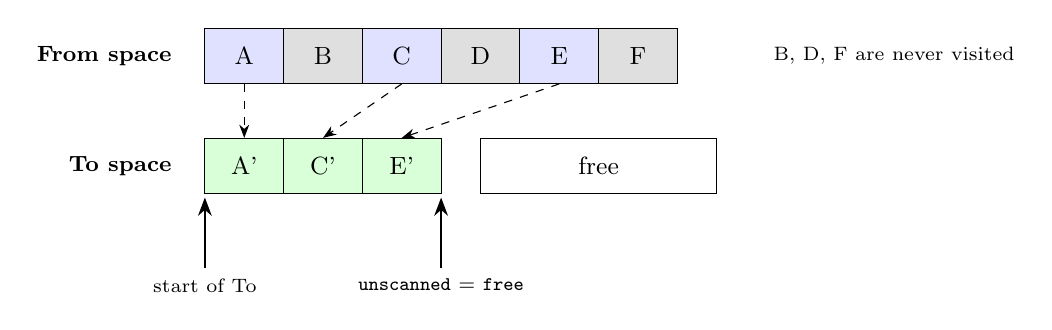
\begin{tikzpicture}[>=Stealth,font=\small]
\node[font=\footnotesize\bfseries,anchor=east] at (-0.8,1.4) {From space};
\node[draw,minimum width=1.00cm,minimum height=0.7cm,fill=blue!12] (fa) at (0.00,1.40) {A};
\node[draw,minimum width=1.00cm,minimum height=0.7cm,fill=gray!25] (fb) at (1.00,1.40) {B};
\node[draw,minimum width=1.00cm,minimum height=0.7cm,fill=blue!12] (fc) at (2.00,1.40) {C};
\node[draw,minimum width=1.00cm,minimum height=0.7cm,fill=gray!25] (fd) at (3.00,1.40) {D};
\node[draw,minimum width=1.00cm,minimum height=0.7cm,fill=blue!12] (fe) at (4.00,1.40) {E};
\node[draw,minimum width=1.00cm,minimum height=0.7cm,fill=gray!25] (ff) at (5.00,1.40) {F};
\node[font=\footnotesize\bfseries,anchor=east] at (-0.8,0) {To space};
\node[draw,minimum width=1.00cm,minimum height=0.7cm,fill=green!15] (ta) at (0.00,0.00) {A'};
\node[draw,minimum width=1.00cm,minimum height=0.7cm,fill=green!15] (tc) at (1.00,0.00) {C'};
\node[draw,minimum width=1.00cm,minimum height=0.7cm,fill=green!15] (te) at (2.00,0.00) {E'};
\node[draw,minimum width=3.0cm,minimum height=0.7cm] at (4.5,0) {free};
\draw[->,dashed] (fa.south) -- (ta.north); \draw[->,dashed] (fc.south) -- (tc.north); \draw[->,dashed] (fe.south) -- (te.north);
\draw[->,thick] (-0.5,-1.3) node[below,font=\scriptsize]{start of To} -- (-0.5,-0.4);
\draw[->,thick] (2.5,-1.3) node[below,font=\scriptsize]{\texttt{unscanned} $=$ \texttt{free}} -- (2.5,-0.4);
\node[font=\scriptsize,anchor=west] at (6.6,1.4) {B, D, F are never visited};
\end{tikzpicture}
\end{document}
